\documentclass[handout]{beamer}
\usepackage{amsmath}
\usepackage{listings}
\usepackage{pgfplots}
\usepackage{graphicx}
\usepackage[default]{sourcecodepro}
\usepackage[default]{sourcesanspro}
\usepackage[T1]{fontenc}
\begin{document}
\title{Zero Intelligence Traders on GPUs with CUDA}
\author{David Prentiss}
\date{\today}

\lstset{
  language = C,
  basicstyle = \fontsize{7.5}{7.7}\selectfont\ttfamily,
  keywordstyle = \color{blue}
}

\frame{\titlepage}

\begin{frame}
  \frametitle{Blocks and Threads}
  \centering
  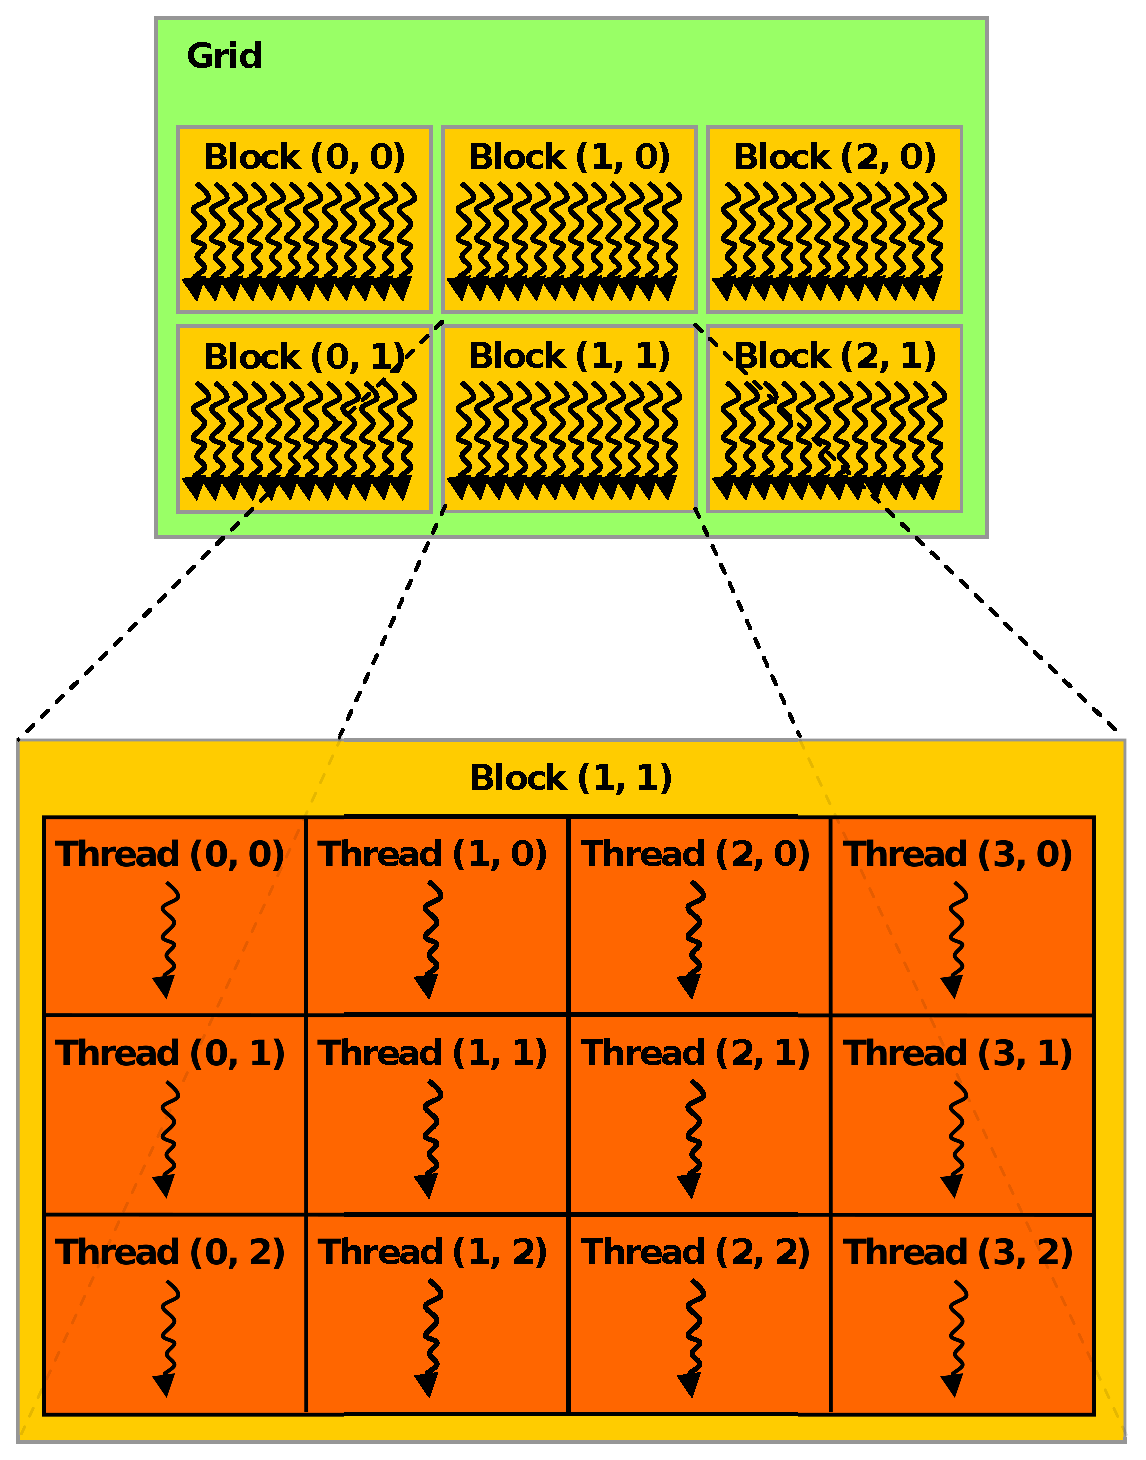
\includegraphics[height=.9\textheight,keepaspectratio]{block-thread.eps}
\end{frame}

\begin{frame}
  \frametitle{Blocks and Threads on Hardware}
  \centering
  \includegraphics[width=\textwidth,keepaspectratio]{Software-Perspective_for_thread_block.jpg}
\end{frame}

\begin{frame}
  \frametitle{Streaming Multiprocessor}
  \centering
  \includegraphics[width=\textwidth,keepaspectratio]{Streaming-Multiprocessor}
\end{frame}

\begin{frame}
  \frametitle{Warp Scheduling}
  \centering
  \includegraphics[width=\textwidth,keepaspectratio]{Warp-Scheduler-Gpu.jpg}
\end{frame}

\begin{frame}
  \frametitle{Example: Dot Product}
  Consider the vectors
  \begin{align*}
    \boldsymbol{a} &= \begin{bmatrix} 3 & 0 & 2 & 1 \end{bmatrix} \\
    \boldsymbol{b} &= \begin{bmatrix} 7 & 6 & 8 & 5 \end{bmatrix}
  \end{align*}
  We want to compute the dot product
  \begin{align*}
    \boldsymbol{c} =
    \boldsymbol{a}\cdot\boldsymbol{b}
    & = \sum_{i=1}^n a_ib_i
  \end{align*}
\end{frame}

\begin{frame}
  \frametitle{Example: Human, SIMD Computers}
  \centering
  \begin{tabular}{cr|c|c|c|c|}
    &\texttt{idx} & 0 & 1 & 2 & 3 \\
    \hline
    &\texttt{a} & 3 & 0 & 2 & 1 \\
    &\texttt{b} & 7 & 6 & 8 & 5 \\
    (0) & \texttt{c} & 0 & 0 & 0 & 0 \\
    (1) & \texttt{c} & 21 & 0 & 16 & 5 \\
    (2) & \texttt{c} & ? & ? & ? & ? \\
    (3) & \texttt{c} & ? & ? & ? & ? \\
  \end{tabular}
  \\
  \vspace{10pt}
  \begin{enumerate}
  \item \texttt{c[idx] = a[idx] * b[idx];}
  \item \texttt{c[idx] = c[idx] + c[(idx+1)\%4];}
  \item \texttt{c[idx] = c[idx] + c[(idx+2)\%4];}
  \end{enumerate}
\end{frame}

\begin{frame}
  \frametitle{Example: Avoiding Race conditions}
  \centering
  \begin{tabular}{cr|c|c|c|c|}
    &\texttt{idx} & 0 & 1 & 2 & 3 \\
    \hline
    &\texttt{a} & 3 & 0 & 2 & 1 \\
    &\texttt{b} & 7 & 6 & 8 & 5 \\
    (0) & \texttt{c} & 0 & 0 & 0 & 0 \\
    (1) & \texttt{c} & 21 & 0 & 16 & 5 \\
    (3) & \texttt{c} & 21 & 16 & 21 & 26 \\
    (5) & \texttt{c} & 42 & 42 & 42 & 42 \\
  \end{tabular}
  \vspace{10pt}
  \begin{enumerate}
  \item \texttt{c[idx] = a[idx] * b[idx];}
  \item \texttt{tmp = c[(idx+1)\%4];}
  \item \texttt{c[idx] = c[idx] + tmp;}
  \item \texttt{tmp = c[(idx+2)\%4];}
  \item \texttt{c[idx] = c[idx] + tmp;}
  \end{enumerate}
\end{frame}

\begin{frame}[fragile]
  \frametitle{Example: \texttt{\_\_syncthreads()}}
  \lstset{
    language = C,
    basicstyle = \ttfamily,
    keywordstyle = \color{blue}
  }
\begin{lstlisting}
int tmp;
c[idx] = a[idx] * b[idx];
__syncthreads();
tmp = c[(idx+1)%4];
__syncthreads();
c[idx] = c[idx] + tmp;
__syncthreads();
tmp = c[(idx+2)%4];
__syncthreads();
c[idx] = c[idx] + tmp;
\end{lstlisting}
\end{frame}

\begin{frame}[fragile]
  \frametitle{Example: Interleaved Reduction}
  \centering
  \begin{tabular}{cr|c|c|c|c|}
    &\texttt{idx} & 0 & 1 & 2 & 3 \\
    \hline
    &\texttt{a} & 3 & 0 & 2 & 1 \\
    &\texttt{b} & 7 & 6 & 8 & 5 \\
    & \texttt{c} & 0 & 0 & 0 & 0 \\
    & \texttt{c} & 21 & 0 & 16 & 5 \\
    (n = 2) & \texttt{c} & \color{red} 21 & 0 & \color{red} 21 & 5 \\
    (n = 4) & \texttt{c} & \color{red} 42 & 0 & 21  & 5 \\
  \end{tabular}
  \vspace{10pt}
  \lstset{
    language = C,
    basicstyle = \ttfamily,
    keywordstyle = \color{blue}
  }
\begin{lstlisting}
int size = 4;
c[idx] = a[idx] * b[idx];
__syncthreads();
for (int n = 2; n < size + 1; n = 2 * n) {
    if (idx % n == 0) {
        c[idx] = c[idx] + c[idx+n-1];
    }
}

\end{lstlisting}
\end{frame}

\begin{frame}
  \frametitle{Title}
\end{frame}

\begin{frame}
  \frametitle{ZI Traders: Threads on GPUs}
  \begin{itemize}
  \item GPUs can be used as many, slower CPUs
  \item We can write a function-for-function clone of the pthreads version in CUDA
  \item As with pthreads, we divide the population into
    subgroups that are executed serially by one thread each
  \item Since data is not needed across threads, data race conditions are not
    a concern
  \item Only a few changes are required...
  \end{itemize}
\end{frame}

\section{Comparing CUDA and pthreads}
\begin{frame}[fragile]
  \frametitle{ZI Traders: Allocating Memory}
  pthreads
\begin{lstlisting}[frame=single]
Agent Buyers[numberOfBuyers];
Agent Sellers[numberOfSellers];
\end{lstlisting}

  CUDA
\begin{lstlisting}[frame=single]
size_t agentSize = numberOfBuyers * sizeof(Agent);
cudaMallocManaged(&Buyers, agentSize);
cudaMallocManaged(&Sellers, agentSize);
...
cudaFree(Buyers);
cudaFree(Sellers);
\end{lstlisting}
  \begin{itemize}
  \item Dynamic allocation
  \item Unified Memory
  \item Can also explicitly copy to device memory
  \item Must free memory after use
  \end{itemize}
\end{frame}

\begin{frame}[fragile]
  \frametitle{ZI Traders: Launching threads}
  pthreads
\begin{lstlisting}[frame=single]
int threadNumber, status;
pthread_t threads[numThreads];
int args[numThreads];

for (threadNumber = 0; threadNumber < numThreads; threadNumber++) {
    args[threadNumber] = threadNumber;
    status = pthread_create(&threads[threadNumber], NULL, DoTrades,
                            &args[threadNumber]);
}
\end{lstlisting}

  CUDA
\begin{lstlisting}[frame=single]
doTrades<<<numBlocks, numThreads>>>(Buyers, Sellers);
\end{lstlisting}
  \begin{itemize}
  \item ``Triple chevrons'' enclose thread dimentions
  \item Parameters follow in parenthesis
  \end{itemize}
\end{frame}

\begin{frame}[fragile]
  \frametitle{ZI Traders: Joining threads}
  pthreads
\begin{lstlisting}[frame=single]
void *threadResult[numThreads];

for (threadNumber = 0; threadNumber < numThreads; threadNumber++) {
    status = pthread_join(threads[threadNumber],
                          &threadResult[threadNumber]);
}
\end{lstlisting}

  CUDA
\begin{lstlisting}[frame=single]
cudaDeviceSynchronize();
\end{lstlisting}
\end{frame}

\begin{frame}[fragile]
  \frametitle{ZI Traders: Concurrent Function}
  pthreads
\begin{lstlisting}[frame=single]
void *DoTrades (void *threadN)
{
    int threadNum = *(int*) threadN;
    ...
    bidPrice = (rand_r(&seeds[threadNum])
        % Buyers[buyerIndex].value) + 1;
    ...
}
\end{lstlisting}

  CUDA
\begin{lstlisting}[frame=single]
__global__ void doTrades(Agent *Buyers, Agent *Sellers)
{
    curandState_t state;
    curand_init(0, 0, 0, &state);

    int threadNum = blockDim.x * blockIdx.x + threadIdx.x;
    ...
    bidPrice = (curand(&state)
        % Buyers[buyerIndex].value) + 1;
    ...
}
\end{lstlisting}
\end{frame}

\begin{frame}
  \centering
  \frametitle{Speedup}
  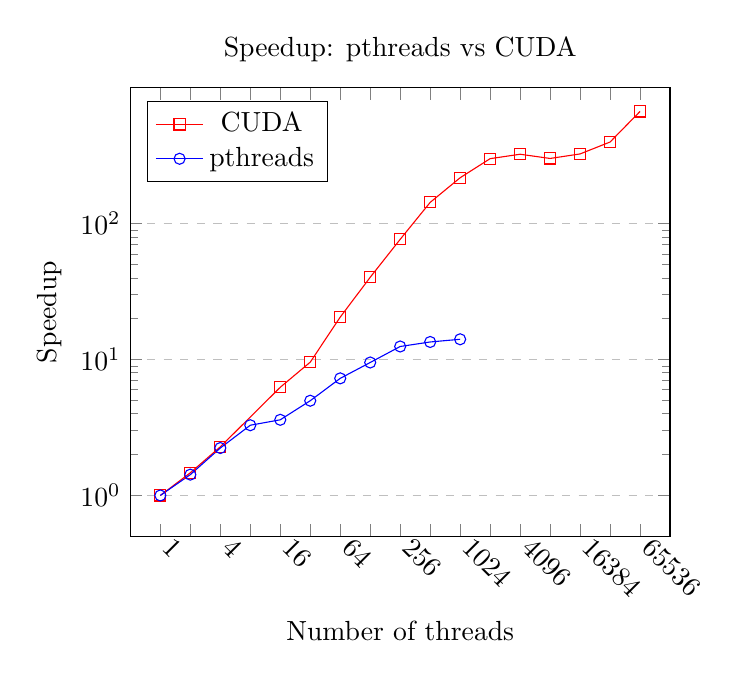
\begin{tikzpicture}
    \begin{axis}[
      title={Speedup: pthreads vs CUDA},
      xlabel={Number of threads},
      ylabel={Speedup},
      ymode=log,
      xmin=0, xmax=18,
      ymin=0, ymax=1000,
      xtick={1,2,3,4,5,6,7,8,9,10,11,12,13,14,15,16,17},
      % xticklabels={1, 2, 4, 8, 16, 32, 64, 128, 256, 512, 1024, 2048, 4096, 8192, 16384, 32768, 65536},
      xticklabels={1, , 4, , 16, , 64, , 256, , 1024, , 4096, , 16384, , 65536},
      xticklabel style = {rotate=-45, anchor=west},
      ytick={1,10,100},
      legend pos=north west,
      ymajorgrids=true,
      grid style=dashed,
      ]

      \addplot[
      color=red,
      mark=square,
      ]
      coordinates {
        (1,1) (2,1.46817178437004) (3,2.27966683380011)
        (5,6.25537598997076)
        (6,9.5750896948336)
        (7,20.5386352699511)
        (8,40.3509893970916)
        (9,76.7700659901252)
        (10,143.551504644803)
        (11,218.036321922191)
        (12,301.29769573665)
        (13,324.737011796832)
        (14,302.330239105228)
        (15,326.415606076669)
        (16,399.371476483461)
        (17,670.493679536725)
      };
      \addlegendentry{CUDA}


      \addplot[
      color=blue,
      mark=o,
      ]
      coordinates {
        (1,1) (2,1.4230249049462) (3,2.23368123893318) (4,3.28693552094917) (5,3.60417185157397) (6,4.97964548239192) (7,7.27522446796857) (8,9.51971038193584) (9,12.4849771438746) (10,13.4781166888948) (11,14.108173590518)
      };
      \addlegendentry{pthreads}

    \end{axis}
  \end{tikzpicture}
\end{frame}

\begin{frame}
  \centering
  \frametitle{Speedup}
  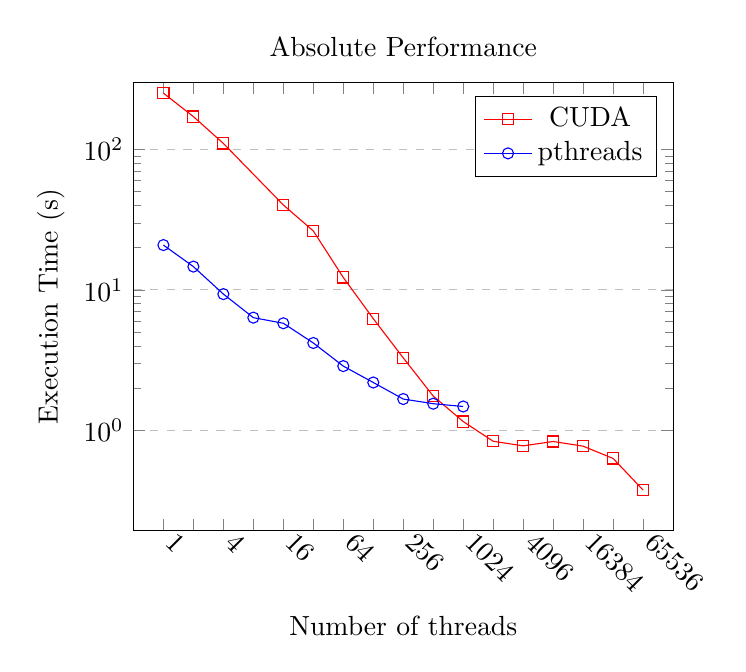
\begin{tikzpicture}
    \begin{axis}[
      ymode = log,
      title={Absolute Performance},
      xlabel={Number of threads},
      ylabel={Execution Time (s)},
      xmin=0, xmax=18,
      ymin=0, ymax=300,
      xtick={1,2,3,4,5,6,7,8,9,10,11,12,13,14,15,16,17},
      xticklabels={1, , 4, , 16, , 64, , 256, , 1024, , 4096, , 16384, , 65536},
      % xticklabels={1, 2, 4, 8, 16, 32, 64, 128, 256, 512, 1024, 2048, 4096, 8192, 16384, 32768, 65536},
      xticklabel style = {rotate=-45, anchor=west},
      ytick={1,10,100},
      legend pos=north east,
      ymajorgrids=true,
      grid style=dashed,
      ]

      \addplot[
      color=red,
      mark=square,
      ]
      coordinates {
        (1,251.8516405)
        (2,171.5409894)
        (3,110.4773894)
        (5,40.2616311)
        (6,26.302797)
        (7,12.2623357)
        (8,6.2415233)
        (9,3.2805969)
        (10,1.754434)
        (11,1.1550903)
        (12,0.8358897)
        (13,0.7755557)
        (14,0.8330349)
        (15,0.7715674)
        (16,0.63062)
        (17,0.3756212)
      };
      \addlegendentry{CUDA}



      \addplot[
      color=blue,
      mark=o,
      ]
      coordinates {
        (1,20.8596189) (2,14.6586464) (3,9.3386731) (4,6.3462209) (5,5.7876316) (6,4.1889767) (7,2.8672131) (8,2.1912031) (9,1.6707775) (10,1.5476657) (11,1.4785485)
      };
      \addlegendentry{pthreads}

    \end{axis}
  \end{tikzpicture}
\end{frame}

\begin{frame}
  \centering
  \frametitle{Speedup}
  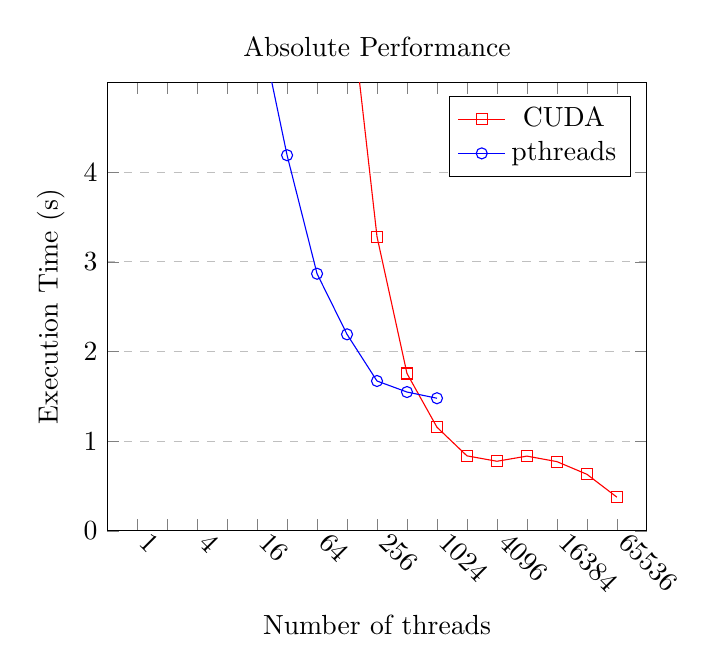
\begin{tikzpicture}
    \begin{axis}[
      title={Absolute Performance},
      xlabel={Number of threads},
      ylabel={Execution Time (s)},
      xmin=0, xmax=18,
      ymin=0, ymax=5,
      xtick={1,2,3,4,5,6,7,8,9,10,11,12,13,14,15,16,17},
      % xticklabels={1, 2, 4, 8, 16, 32, 64, 128, 256, 512, 1024, 2048, 4096, 8192, 16384, 32768, 65536},
      xticklabels={1, , 4, , 16, , 64, , 256, , 1024, , 4096, , 16384, , 65536},
      xticklabel style = {rotate=-45, anchor=west},
      ytick={0,1,2,3,4},
      legend pos=north east,
      ymajorgrids=true,
      grid style=dashed,
      ]

      \addplot[
      color=red,
      mark=square,
      ]
      coordinates {
        (1,251.8516405)
        (2,171.5409894)
        (3,110.4773894)
        (5,40.2616311)
        (6,26.302797)
        (7,12.2623357)
        (8,6.2415233)
        (9,3.2805969)
        (10,1.754434)
        (11,1.1550903)
        (12,0.8358897)
        (13,0.7755557)
        (14,0.8330349)
        (15,0.7715674)
        (16,0.63062)
        (17,0.3756212)
      };
      \addlegendentry{CUDA}



      \addplot[
      color=blue,
      mark=o,
      ]
      coordinates {
        (1,20.8596189) (2,14.6586464) (3,9.3386731) (4,6.3462209) (5,5.7876316) (6,4.1889767) (7,2.8672131) (8,2.1912031) (9,1.6707775) (10,1.5476657) (11,1.4785485)
      };
      \addlegendentry{pthreads}

    \end{axis}
  \end{tikzpicture}
\end{frame}

\end{document}